\documentclass[tikz,border=0pt]{standalone}%
\usepackage{tikz-cd}
\usepackage{ifthen}
\usepackage{amsmath}
\usetikzlibrary{arrows,calc,intersections,shapes}
\begin{document}
%---------------------------------------------------------------
        %% GRNN
        %-----------------------------------------
        %% linkes Bild
        \begin{tikzpicture}[>=stealth', node distance=\layersep cm, shorten >=1pt]
        \def\layersep{1.8}          % vertikal distance between the layers
        \def\neuronsep{1.8}         % Horizontal distance between neurons
        \def\dlsize{2}              % distance between node and layer lable
        \def\inout{\layersep*.65}   % Size of in- and output-arrow
        \def\siz{.8}                % neuronsize
        \def\y{5}                   % Start of the most upper layer
        \def\ni{3}                  % Amount of input neurons
        \def\nh{4}                  % Amount of pattern neurons
        \def\ns{2}                  % Amount of hidden neurons
        \def\no{1}                  % Amount of output neurons
        \tikzstyle{neuron}=[circle,draw=black,minimum size=\siz cm,inner sep=2pt]
        \tikzstyle{annot} = [text width=7em, text centered]
        \tikzset{fontscale/.style = {font={\fontsize{#1pt}{#1pt}\selectfont}}}
        \tikzset{
            ident/.pic={
                \draw[semithick] (-\siz/#1,-\siz/#1) -- (\siz/#1,\siz/#1);
            }
        }
        \newcommand{\neurono}[3][]{%
            \ifthenelse{\equal{#3}{0}}{%
                \node[neuron,circle split,inner sep=.8pt,fontscale=6] (#1) at (#2)
                    { $\mathbf{||x\mathord{,}x'||}$ \nodepart{lower} };
                    
                \node[fontscale=6] at ($(#2.lower)-(0,\siz/4)$){\textbf{Exp.}};
            }{
                \ifthenelse{\equal{#3}{1}}{
                \node[neuron] (#1) at (#2) {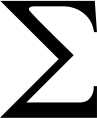
\includegraphics[width=0.3cm]{Bilder/Sigma.png}};
                }{
                \node[neuron,fontscale=15] (#1) at (#2){$\divisionsymbol$}; % if physics package is loaded use \divisionsymbol instead of \div 
                }
            }
        }
        % Draw the left input layer nodes
            \foreach \name / \xn in {1,...,\ni}{
                \node[neuron,fontscale=15] (Il-\name) at (\xn*\neuronsep-\neuronsep,\y) {$i_{\xn}$};
                \node[above of=Il-\name, node distance=\inout cm] (Inl-\name) {};
                \draw [->,arrows={-Stealth[length=7pt]},densely dotted] (Inl-\name) edge (Il-\name);
            }
        % Draw the pattern layer nodes
            \foreach \name / \xn in {1,...,\nh}{
                \node[neuron] (Hl-\xn) at ({(\ni-1)*\neuronsep/2-\neuronsep/2*(\nh-1)+(\xn-1)*\neuronsep},\y-\layersep) [fontscale=15] {$m_{\xn}$};
                \node[node distance=\inout cm, below of=Hl-\xn] (Hnl) {};
        % Connect every node in the input layer with the pattern layer
            \foreach \source in {1,...,\ni}
                \draw [->,arrows={-Stealth[length=7pt]}] (Il-\source) edge (Hl-\xn);}
        % Draw the summation layer nodes
            \foreach \name / \xn in {1,...,\ns}{
                \node[neuron] (Sl-\xn) at ({(\ni-1)*\neuronsep/2-\neuronsep/2*(\ns-1)+(\xn-1)*\neuronsep},\y-2*\layersep) [fontscale=15] {$s_{\xn}$};
                \node[node distance=\inout cm, below of=Sl-\xn] (Snl) {};
        % Connect every node in the pattern layer with the summation layer
            \foreach \source in {1,...,\nh}
                \draw [->,arrows={-Stealth[length=7pt]}] (Hl-\source) edge (Sl-\xn);}
        % Draw the output layer nodes
            \foreach \name / \xn in {1,...,\no}{
                \node[neuron] (Ol-\xn) at ({(\ni-1)*\neuronsep/2-\neuronsep/2*(\no-1)+(\xn-1)*\neuronsep},\y-3*\layersep) [fontscale=15] {$\Omega_{\xn}$};
                \node[node distance=\inout cm, below of=Ol-\xn] (Onl) {};
                \draw [->,arrows={-Stealth[length=7pt]},densely dotted] (Ol-\xn) edge (Onl);
        % Connect every node in the summation layer with the output layer
            \foreach \source in {1,...,\ns}
                \draw [->,arrows={-Stealth[length=7pt]}] (Sl-\source) edge (Ol-\xn);}
        % Annotate the layers
            \def\lni{Eingabe- schicht}                      % Lable of input layer
            \def\lnh{Musterschicht}                       % Lable of pattern layer
            \def\lns{Summierungs- schicht}                  % Lable of summation layer
            \def\lno{Ausgabe- schicht}                      % Lable of output layer
            \ifthenelse{\ni>\nh \AND \ni>\ns}{
                \node[annot,right of=Il-\ni, node distance=\dlsize cm] (il) {\textbf{\lni}};
                \node[annot,below of=il] (hl) {\textbf{\lnh}};
                \node[annot,below of=hl] (sl) {\textbf{\lns}};
            }{
                \ifthenelse{\nh>\ns}{
                    \node[annot,right of=Hl-\nh, node distance=\dlsize cm] (hl) {\textbf{\lnh}};
                    \node[annot,above of=hl] (il) {\textbf{\lni}};
                    \node[annot,below of=hl] (sl) {\textbf{\lns}};
                }{
                    \node[annot,right of=Sl-\ns, node distance=\dlsize cm] (sl) {\textbf{\lns}};
                    \node[annot,above of=sl] (hl) {\textbf{\lnh}};
                    \node[annot,above of=hl] (il) {\textbf{\lni}};
                }
                
            }
                \node[annot,below of=sl] {\textbf{\lno}};
        %-----------------------------------------
        %% rechtes Bild
        % Draw the right input layer nodes
                \coordinate (tIr) at ($(il)-(Il-\ni)$);
                \coordinate (ttIr) at (tIr |- 0,0);
                \coordinate (Ir) at ($(il)+(ttIr)$);
            \foreach \name / \xn in {1,...,\ni}{
        % This is the same as writing \foreach \name / \y in {1/1,2/2,3/3,4/4}
                \node[neuron] (Ir-\name) at ($(Ir)+(\xn*\neuronsep-\neuronsep,0)$) {};
                \node[above of=Ir-\name, node distance=\inout cm] (Inr-\name) {};
                \pic at (Ir-\name) {ident=4};
                \draw [->,arrows={-Stealth[length=7pt]},densely dotted] (Inr-\name) edge (Ir-\name);}
        % Draw the right pattern layer nodes
            \foreach \name / \xn in {1,...,\nh}{
                \neurono[Hr-\xn]{$(Ir)+({(\ni-1)*\neuronsep/2-\neuronsep/2*(\nh-1)+(\xn-1)*\neuronsep},-\layersep)$}{0}
                \node[node distance=\inout cm, below of=Hr-\xn] (Hnr) {};
        % Connect every node in the input layer with the pattern layer
                \foreach \source in {1,...,\ni}
                \draw [->,arrows={-Stealth[length=7pt]}] (Ir-\source) edge  (Hr-\xn);}
        % Draw the right summation layer nodes
            \foreach \name / \xn in {1,...,\ns}{
                \neurono[Sr-\xn]{$(Ir)+({(\ni-1)*\neuronsep/2-\neuronsep/2*(\ns-1)+(\xn-1)*\neuronsep},-2*\layersep)$}{1}
                \node[node distance=\inout cm, below of=Sr-\xn] (Snr) {};
        % Connect every node in the pattern layer with the summation layer
                \foreach \source in {1,...,\nh}
                \draw [->,arrows={-Stealth[length=7pt]}] (Hr-\source) edge  (Sr-\xn);}
            \foreach \xn in {1}{
                \foreach \source in {1,...,\nh}
                    \node[fill=white,inner sep=1pt,fontscale=10] at ($(Hr-\source)!.3+.1!(Sr-\xn)$) {$y_{\source}$};} 
        % Draw the right output layer nodes
            \foreach \name / \xn in {1,...,\no}{
                \neurono[Or-\xn]{$(Ir)+({(\ni-1)*\neuronsep/2-\neuronsep/2*(\no-1)+(\xn-1)*\neuronsep},-3*\layersep)$}{6}
                \node[node distance=\inout cm, below of=Or-\xn] (Onr) {};
                \draw [->,arrows={-Stealth[length=7pt]},densely dotted] (Or-\xn) edge (Onr);
        % Connect every node in the summation layer with the output layer
            \foreach \source in {1,...,\ns}
                \draw [->,arrows={-Stealth[length=7pt]}] (Sr-\source) edge  (Or-\xn);}
        \end{tikzpicture}
\end{document}}